% Owned contribution: geometry_frontiers. Frozen delivery, 2026-10-29.
% Requires the root article's standard theorem environments and macros.
% Citation keys: HK2017, HKO2026. Certificate names are relative placeholders
% for the root's retained affine-hko-compressed packet.
\section{The pentagon counterexample in its full affine class}
\label{sec:affine-hko}

The pentagon counterexample is naturally presented as a Lagrangian product.
An arbitrary linear image need not retain that feature: its two factor
planes can cease to be Lagrangian. We optimize over this larger class.
The proof records all affine deformations by a skew form, then projects the
resulting six-dimensional capacity constraint to a three-dimensional convex
body. A small exact certificate places that projection inside the unit ball.

Let $P\subset\mathbb R^2$ be the regular pentagon with vertices
$(\cos(2\pi k/5),\sin(2\pi k/5))$, and put
\[
 H=P\times R(-\pi/2)P\subset\mathbb R^2_q\times\mathbb R^2_p.
\]
Haim--Kislev and Ostrover computed
$\rho(H)=(3+\sqrt5)/5$~\cite{HKO2026}.

\begin{theorem}[Affine optimality of the HKO product]
\label{thm:affine-hko}
For every $A\in GL(4,\mathbb R)$,
\[
 \rho(AH)\leq\rho(H)=\frac{3+\sqrt5}{5}.
\]
Equality holds if and only if $AH=\lambda SH$ for some $\lambda>0$ and
$S\in\operatorname{Sp}(4,\mathbb R)$. The same statement holds after
allowing translations of the bodies.
\end{theorem}

The class includes separate affine changes of the two pentagon factors and
linear maps mixing their planes. It does not include general perturbations
of the ten facets or bodies with a different affine shape.

\subsection{Affine deformation through an action body}
\label{subsec:affine-action-body}

Use product coordinates and the matrix
\[
 J=\begin{pmatrix}0&I_2\\-I_2&0\end{pmatrix},
 \qquad \omega_0(a,b)=a^{\mathsf T}Jb.
\]
Identify a skew matrix $\Omega$ with
\[
 x=(x_{01},x_{02},x_{03},x_{12},x_{13},x_{23})
   =(\Omega_{01},\Omega_{02},\Omega_{03},\Omega_{12},\Omega_{13},\Omega_{23}),
\]
and write
\begin{equation}
 \mathfrak p(x)=-\Pf(\Omega)
 =x_{02}x_{13}-x_{01}x_{23}-x_{03}x_{12}.
 \label{eq:affine-pfaffian}
\end{equation}
In particular, $J$ has coordinates $(0,1,0,0,1,0)$ and
$\mathfrak p(J)=1$. The minus sign comes from the product-coordinate order.

For a bounded full-dimensional polytope
$K=\{z:a_i\cdot z\leq1\}$, define its \emph{action body}
$\mathcal W_K\subset\bigwedge^2\mathbb R^4$ as the convex hull of
\begin{equation}
 b_{\sigma,\beta}
 =\sum_{i<j}\beta_i\beta_j
     \bigl(a_{\sigma(i)}\wedge a_{\sigma(j)}\bigr),
 \quad
 \beta_i\geq0,\quad \sum_i\beta_i=1,\quad
 \sum_i\beta_i a_{\sigma(i)}=0,
 \label{eq:affine-action-witness}
\end{equation}
where $\sigma$ ranges over words of distinct facets. The coordinate of
$a\wedge b$ indexed by $ij$ is $a_i b_j-a_j b_i$, so its pairing with $x$
is $a^{\mathsf T}\Omega b$.

\begin{lemma}[Affine capacity formula]
\label{lem:affine-action-body}
The body $\mathcal W_K$ is compact, centrally symmetric, and has nonempty
interior. Its support function satisfies
\begin{equation}
 c_{\EHZ}(AK)
 =\frac{1}{2h_{\mathcal W_K}(A^{-1}JA^{-\mathsf T})}
 \qquad(A\in GL(4,\mathbb R)).
 \label{eq:affine-capacity-formula}
\end{equation}
For $\det A>0$ and $x$ the coordinates of $A^{-1}JA^{-\mathsf T}$,
\begin{equation}
 \rho(AK)=\frac{\mathfrak p(x)}
 {8\Vol_4(K)h_{\mathcal W_K}(x)^2}.
 \label{eq:affine-ratio-formula}
\end{equation}
\end{lemma}

\begin{proof}
Each word has a compact feasible weight set, and there are finitely many
words. Reversing the word and its weights negates its bivector, proving
central symmetry. Under $K\mapsto AK$, the normals become
$A^{-\mathsf T}a_i$, while the feasible weights remain exactly the same.
Their ordered action is the pairing in
\eqref{eq:affine-action-witness} with $A^{-1}JA^{-\mathsf T}$.
The Haim--Kislev formula~\cite{HK2017} therefore gives
\eqref{eq:affine-capacity-formula}. Its source convention pairs the later
facet with the earlier one; reversing every word and its weights gives the
displayed convention. Inserting or deleting zero weights identifies the
subset-word formula with the full-permutation formula.

To prove nonempty interior, choose a strictly positive feasible vector on
all the normals. Such a vector exists because the normals positively span
$\mathbb R^4$, so zero lies in the interior of their convex hull. If a skew
form annihilates $\mathcal W_K$, every ordering of this vector has zero
action. Interchanging adjacent facets $i,j$ changes the action by
$2\beta_i\beta_j a_i^{\mathsf T}\Omega a_j$. All these pairings must
vanish. Since the normals span $\mathbb R^4$, the form is zero. Thus
$\mathcal W_K$ spans the bivector space; its symmetry gives nonempty
interior. In particular its support function is a norm.

Finally,
\[
 \Pf(A^{-1}JA^{-\mathsf T})=\frac{\Pf(J)}{\det A}=-\frac1{\det A}.
\]
Combining this identity with $\Vol_4(AK)=\det A\Vol_4(K)$ proves
\eqref{eq:affine-ratio-formula}.
\end{proof}

The lemma replaces optimization over matrices $A$ by optimization of a
quadratic Pfaffian on the polar of a fixed convex body. The capacity
constraint retains its full meaning even when the factor planes are no
longer Lagrangian. A finite collection of feasible witnesses gives only
some supporting inequalities of this polar, which is sufficient for an
upper bound if those inequalities have the right geometry.

\subsection{A three-dimensional projection inside the unit ball}

For the rest of the section write $\mathcal W=\mathcal W_H$. Set
\[
 t=\tan(\pi/5),\quad s=\sqrt5=\frac{5-t^2}{2},\quad
 c_0=5t-\frac{t^3}{2},\quad q_0=\frac1{2c_0},\quad
 V_0=\frac{25(5+s)}{32}.
\]
Here $c_0=c_{\EHZ}(H)$ and $V_0=\Vol_4(H)$, so
\begin{equation}
 \frac1{8V_0q_0^2}=\frac{3+s}{5}.
 \label{eq:affine-hko-normalization}
\end{equation}
Consider the full normalized action polar
\[
 \mathcal C=\{x:h_{\mathcal W}(x)\leq q_0\}.
\]
Define two linear maps to $\mathbb R^3$ by
\begin{align}
 U(x)&=\frac12(x_{02}+x_{13},\ x_{03}-x_{12},\ x_{01}-x_{23}),
 \label{eq:affine-U}\\
 V(x)&=\frac12(x_{02}-x_{13},\ x_{03}+x_{12},\ x_{01}+x_{23}).
 \nonumber
\end{align}
These are coordinates on the two three-dimensional summands of the skew
forms. Direct expansion gives
\begin{equation}
 \mathfrak p(x)=|U(x)|^2-|V(x)|^2.
 \label{eq:affine-split-norm}
\end{equation}
Consequently a unit-ball bound on $U(\mathcal C)$ controls the Pfaffian.

The outer body used for that bound is elementary. Let $D$ be the regular
20-gon with vertices at angles $k\pi/10$, of circumradius one, and let
$E\subset D$ be the regular decagon consisting of the even-indexed vertices.
Put
\begin{equation}
 a=\frac{5-\sqrt5}{4},\qquad r=\frac{143}{200},\qquad
 T=\conv\bigl((E\times\{0\})\cup(rD\times\{a\})
                         \cup(rD\times\{-a\})\bigr).
 \label{eq:affine-outer-body}
\end{equation}
The rational number $r$ supplies convenient slack in the certificate; it
is not asserted to be an optimal auxiliary constant.

\begin{figure}[tb]
 \centering
 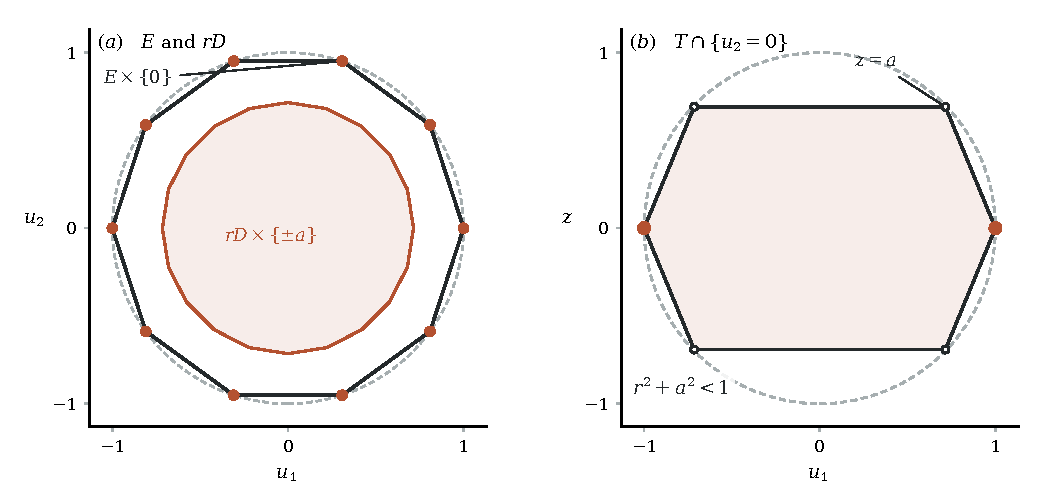
\includegraphics[width=.96\linewidth]{figures/affine-outer-body.pdf}
 \caption{The outer projection body $T$: its middle and end polygons in
 plan view, and an axial section inside the unit-ball section. Only the
 ten equatorial vertices meet the sphere.}
 \label{fig:affine-outer}
\end{figure}


\begin{proposition}[Projection certificate]
\label{prop:affine-projection}
The full action polar satisfies
\[
 U(\mathcal C)\subset T\subset\overline B^3(1).
\]
Moreover $T\cap S^2$ consists of exactly the ten vertices of
$E\times\{0\}$.
\end{proposition}

\begin{proof}
First describe $T$ without computation. Since $rD\subset E$, its slice at
height $|z|=a\tau$, for $0\leq\tau\leq1$, is
$(1-\tau)E+\tau rD$. One way to verify this slice identity is to replace
a mixture of the upper and lower copies of $rD$ by a point of $E$ at
height zero; the remaining mixture has the stated form.
The edge normals of the planar Minkowski sum are the union of the edge
normals of its two summands. Thus a complete halfspace description of $T$
is $|z|\leq a$, together with
\begin{equation}
 n\cdot u+\frac{d_0-d_1}{a}|z|\leq d_0,
 \qquad d_0=h_E(n),\quad d_1=rh_D(n),
 \label{eq:affine-outer-halfspaces}
\end{equation}
for every edge-normal direction of $E$ or $D$. There are $62$ halfspaces:
two horizontal ones and two for each of $30$ planar directions.
For exact coordinates, the edge normals of $E$ can be taken to be the odd
vertices of $D$, and those of $D$ to be sums of adjacent vertices of $D$.

The vertices in the middle level of $T$ have norm one, whereas all the
vertices in its upper and lower levels satisfy
\[
 |(ru,\pm a)|^2=r^2+a^2<1.
\]
Convexity proves $T\subset\overline B^3(1)$. Strict convexity of the ball
shows that its unit-sphere contacts are exactly the ten middle vertices.

It remains to place $U(\mathcal C)$ in these halfspaces. The finite
certificate described below supplies $18$ feasible action bivectors
$q_0b_j\in\mathcal W$. Write $Lx=U(x)$. For four representative
halfspaces $h_0+h\cdot y\geq0$, with $h_0>0$, it gives coefficients
$\lambda_j\geq0$ satisfying
\begin{equation}
 \sum_j\lambda_j=1,\qquad
 \sum_j\lambda_jb_j=-\frac{h^{\mathsf T}L}{h_0}.
 \label{eq:affine-dual-certificate}
\end{equation}
Every $x\in\mathcal C$ satisfies $b_j\cdot x\leq1$. Hence
\eqref{eq:affine-dual-certificate} implies the representative halfspace
inequality at $U(x)$.

The remaining halfspaces follow by symmetry. The projection
$U(\mathcal C)$ is invariant under the group generated by
\[
 (u,z)\longmapsto(R(2\pi/5)u,z),\qquad
 (u_1,u_2,z)\longmapsto(u_1,-u_2,z),\qquad
 y\longmapsto-y.
\]
Indeed, the first map is induced by congruence of $\Omega$ with the
$-2\pi/5$ rotation of the $q$ pentagon. The second is induced by the
negative of congruence with
$\operatorname{diag}(1,-1,-1,1)$, the simultaneous horizontal reflection
of the $q$ pentagon and vertical reflection of its partner. The last is
$\Omega\mapsto-\Omega$. The two congruences permute the facet normals
of $H$, and therefore permute the feasible words defining $\mathcal W$;
negation preserves its support function by word reversal. Substitution
in~\eqref{eq:affine-U} gives the claimed maps on $U$.
The four representatives have orbits of sizes $2,20,20,20$, covering all
$62$ halfspaces. The exact verification also checks these normal
permutations, projection identities, and orbit coverage.

The symmetry argument applies to the \emph{full} action polar
$\mathcal C$. The polyhedron defined only by the selected $18$ witness
inequalities need not be invariant under this group. No such invariance
is used. This proves $U(\mathcal C)\subset T$.
\end{proof}

\subsection{The finite predicate and its reproduction}
\label{subsec:affine-certificate}

All finite data lie in the ordered field
$F=\mathbb Q(t)$, where $t^4-10t^2+5=0$ and $0<t<1$. To specify the
geometry used by the certificate, put
\[
 \alpha=\frac{3-s}{2},\qquad \beta=\frac{t(1+s)}2,
 \qquad \delta=s-1.
\]
Define the five planar normals
\[
 u_0=(1,t),\quad u_1=(-\alpha,\beta),\quad u_2=(-\delta,0),\quad
 u_3=(-\alpha,-\beta),\quad u_4=(1,-t).
\]
The ten four-dimensional normals are
$a_i=(u_i,0)$ and $a_{5+i}=(0,R(-\pi/2)u_i)$ for $0\leq i<5$.
For each of the $18$ witnesses the verifier checks distinctness of the
facet indices, nonnegativity and normalization of the weights, closure,
and the exact bivector identity~\eqref{eq:affine-action-witness}.
It then checks the four positive relations
\eqref{eq:affine-dual-certificate}. The words and field coefficients are
stored in \path{certificates/affine-hko/certificate.json}; they are finite proof
inputs rather than requests to run an optimizer.

For a compact description of the four relations, let
$C=\cos(\pi/10)$, $S=\sin(\pi/10)$ and $\eta=S/(1+C)$.
Table~\ref{tab:affine-four-relations} gives the representative inequalities,
their support sizes, and simple exact lower bounds on every nonzero weight.
The first relation averages the two pure-factor five-facet witnesses with
weights $1/2,1/2$. The remaining coefficients are longer elements of $F$;
their complete values are retained in the certificate.

\begin{table}[ht]
\centering
\small
\begin{tabular}{@{}lrrr@{}}
\toprule
Representative halfspace in $(u_1,u_2,z)$
 & Witnesses & Weight lower bound & Orbit size\\
\midrule
$a+z\geq0$ & 2 & $1/2$ & 2\\
$C-u_2+(C-r)z/a\geq0$ & 4 & $1/40$ & 20\\
$1-u_1-\eta u_2+(1-r)z/a\geq0$ & 6 & $1/200$ & 20\\
$1-u_1-\eta u_2-(1-r)z/a\geq0$ & 6 & $1/30$ & 20\\
\bottomrule
\end{tabular}
\caption{Four exact convex combinations imply the complete outer-body
containment by symmetry. The bounds in the third column are not substitutes
for the exact identities.}
\label{tab:affine-four-relations}
\end{table}

The standalone SageMath program verifies the finite data from one JSON
input file. It reconstructs the facet normals,
all witness bivectors, the outer vertices and halfspaces, and the symmetry
actions. It accepts exactly the predicates used above: $18$ feasible
witnesses, four positive relations, coverage of $62$ halfspaces, and the
sphere bounds for $50$ outer vertices with precisely ten unit contacts.
It requires neither numerical optimization nor an external polyhedral
hull computation. Run \path{certificates/affine-hko/verify.py} with a
Python interpreter providing \texttt{sage.all}; it reads the sibling JSON
and records an execution summary. A successful run validates the
finite predicates; the slice argument, symmetry implication, and affine
capacity reduction are the mathematical steps proved in this section.

\subsection{Proof of the sharp bound and equality}

\begin{proof}[Proof of Theorem~\ref{thm:affine-hko}]
First suppose $\det A>0$ and let
$x=A^{-1}JA^{-\mathsf T}$ in skew-form coordinates. Put
$q=h_{\mathcal W}(x)/q_0>0$. By definition $x/q\in\mathcal C$, so
Proposition~\ref{prop:affine-projection} and
\eqref{eq:affine-split-norm} give
\[
 \mathfrak p(x)=|U(x)|^2-|V(x)|^2\leq |U(x)|^2\leq q^2.
\]
Equations~\eqref{eq:affine-ratio-formula} and
\eqref{eq:affine-hko-normalization} prove the claimed upper bound.

If equality holds, both inequalities are equalities. Thus $V(x)=0$, and
$U(x)/q$ is one of the ten unit-sphere contacts of $T$. Consequently
$x/q$ has zero same-factor entries and cross block
\begin{equation}
 \begin{pmatrix}
 \cos(k\pi/5)&\sin(k\pi/5)\\
 -\sin(k\pi/5)&\cos(k\pi/5)
 \end{pmatrix},\qquad k=0,\ldots,9.
 \label{eq:affine-equality-forms}
\end{equation}
Each is $T_0^{-1}JT_0^{-\mathsf T}$ for a linear automorphism $T_0$ of
$H$. Rotations by $2\pi/5$ in one factor give five of the forms; the
simultaneous factor reflections used above preserve $H$ and send $J$ to
$-J$, giving the other five. Therefore
\[
 A^{-1}JA^{-\mathsf T}=qT_0^{-1}JT_0^{-\mathsf T}.
\]
The matrix $S_0=\sqrt q\,AT_0^{-1}$ satisfies $S_0JS_0^{\mathsf T}=J$
and is symplectic. Hence $AH=q^{-1/2}S_0H$.
Conversely, symplectic images and positive dilations preserve $\rho$.

Finally, if $\det A<0$, compose $A$ on the right with
$\operatorname{diag}(1,-1,1,1)$. This is a determinant
$-1$ automorphism of $H$, so it changes the determinant sign without
changing $AH$. The positive-determinant argument applies. Translation
invariance gives the last assertion.
\end{proof}
